\chapter{Category Theory}\label{app:category-theory}

Category theory is a powerful mathematical framework, defined by~\cite{Eilenberg1945}, that provides an abstract way to reason about mathematical structures and the relationships between them.

Categories are particularly useful in Computer Science, having several applications such as design of programming languages, implementation techniques, semantic models, concurrency models, type theory, among others~\cite{Pierce1991}.

Category theory is also the basis for graph transformation systems, which is central to the work proposed in this thesis. Therefore, we present a brief introduction of the field and basic categorial constructions that will be necessary in this work.

\begin{definition}[Category]\label{def:category} A category \cat{C} consists of a collection of \emph{objects} and a collection of \emph{arrows} between objects (also called \emph{morphisms}) such that:

  \begin{enumerate}
    \item for all arrows $f : A \rightarrow B$, $g : B \rightarrow C$ and
$h : C \rightarrow D$, with objects $A,B,C,D$ not necessarily distinct, the composition of arrows is associative:

  $h \circ (g \circ f) = (h \circ g) \circ f$;
    \item for every object $A$ there is an \emph{identity} arrow $id_A : A \rightarrow A$ such that for any arrow $f : A \rightarrow B$:

  $id_B \circ f = f$ and $f \circ id_A = f$.
  \end{enumerate}
\end{definition}

\begin{example}[Category of Sets] \cat{Set} is the category whose objects are \emph{sets} and the arrows and the arrows are \emph{total functions} between sets. \important{I did not understand the first piece of the note}
\end{example}

\begin{definition}[Diagram] Given a category \cat{C}, a diagram in \cat{C} is a collection of vertices and directed edges such that, if an edge in the diagram is named with an arrow $f$ and $f$ has domain $A$ and codomain $B$, then the outgoing vertex of the edge must be named $A$ and the incoming vertex $B$.

  A diagram is said to \emph{commute} if, for every pair of objects $A,B$, all the paths in the diagram from $A$ to $B$ are equal. In other words, each path in the diagram determines an arrow and these arrows are equal in \cat{C}. If the following diagram commutes than we can say that \mbox{$g' \circ f = f' \circ g$}.

\diagram{
  A\ar[r]^{f}\ar[d]_{g} & Y\ar[d]^{g'}\\
  X\ar[r]_{f'} & B
}

\end{definition}

\begin{definition}[Monomorphism, Epimorphism and Isomorphism] An arrow \mbox{$f : B \rightarrow C$} in a category \cat{C} is said to be a \emph{monomorphism} if, for any pair of arrows $g : A \rightarrow B$ and $h : A \rightarrow B$, we have that $f \circ g = f \circ h \Rightarrow g = h$.

\diagram{
  A\ar@<.5ex>[r]^{g}\ar@<-.5ex>[r]_{h} & B\ar[r]^{f} & C
}

  An arrow \morph{f}{A}{B} is said to be an \emph{epimorphism} if, for any pair of arrows \morph{g}{B}{C}, \morph{h}{B}{C}, we have that \mbox{$g \circ f = h \circ f \Rightarrow g = h$}.

\diagram{
  A\ar[r]^{f} & B\ar@<.5ex>[r]^{g}\ar@<-.5ex>[r]_{h} & C
}

  An arrow \morph{f}{A}{B} is an \emph{isomorphism} if there is an arrow \morph{f^{-1}}{B}{A}, the \emph{inverse} of $f$, such that \mbox{$f^{-1} \circ f = id_A$} and \mbox{$f \circ f^{-1} = id_B$}


\diagram{ 
  A\ar@<.5ex>[r]^{f} & B\ar@<.5ex>[l]^{f^{-1}}
}
\end{definition}

\iffalse
\begin{example}[Monomorphism, Epimorphism and Isomorphism Examples]

  In \cat{Set}, the monomorphism, epimorphism and isomorphism concepts correspond to injective, surjective and bijective functions, respectively.\tinytodo{put examples}

  \tinytodo{explain ``up to isomorphism''}

\end{example}
\fi

\section*{Categorial Constructions}

Here we present basic categorial constructions that are used throughout in this work. Notice that this is not an extensive list, we present only the constructions necessary to our scope. For a more in-depth explanation of Category Theory and its application in Computer Science refer to~\cite{Pierce1991}.

\begin{definition}[Coproduct] Given two objects $A$ and $B$, their \emph{coproduct} (also called \emph{categorical sum}) is an object $A+B$ and two injection arrows \morph{i_A}{A}{A+B} and \morph{i_B}{B}{A+B} such that, for any other object $X$ and pair of arrows \morph{f}{A}{X} and \morph{g}{B}{X}, there is one unique arrow \morph{!}{A+B}{X} such that the following diagram commutes:

\diagram{
  A\ar[r]^{i_A}\ar[dr]_{f} & A+B\ar@{.>}[d]^{!} & B\ar[l]_{i_B}\ar[dl]^{g}\\
    & X   &
}

\end{definition}

\begin{example}[Coproducts in \cat{Set}] Coproducts can be used to generalize the notion of disjoint union. Figure~\ref{fig:gts:coproduct} shows an example of it in the category \cat{Set}\footnote{The morphisms are represented in an expanded notation to explicitly show how the mappings were done.}. Having the sets $A = \{1,2,3\}$ and $B = \{1,2\}$ as objects, we have that the set $A+B$ together with morphisms $i_A$ and $i_B$ is their coproduct: all elements of $A$ and $B$ are mapped to $A+B$, no elements from the source objects are identified in the target, and it is possible to find a unique function from $A+B$ to any other candidate satisfying the commutative restriction.

\begin{figure}[!ht]
  \centering
  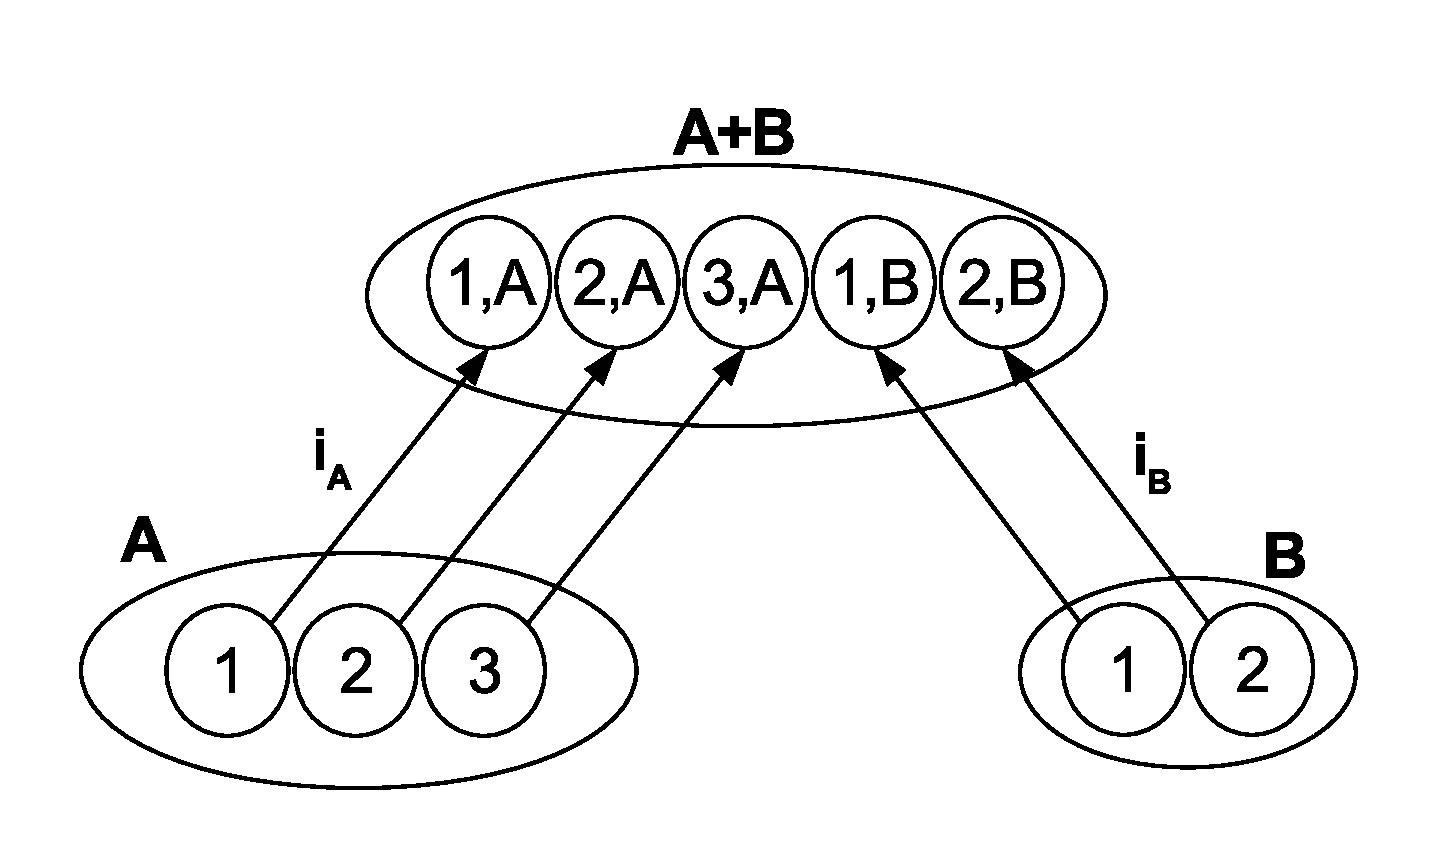
\includegraphics[scale=0.4]{images/gts/coproduct-open}
  \caption{A coproduct in \cat{Set} \important{name the morphisms}}\label{fig:gts:coproduct}
\end{figure}

Notice that $(A+B)' = \{(1,0),(2,0),(3,0),(1,1),(2,1)\}$ or $(A+B)'' = \{a,b,c,d,e\}$ or any other set with five elements would be equally valid as coproducts for this case. This is due to the fact the categories deal with their objects up to isomorphism, i.e. all this objects have the same format regardless of their internal representations.
\end{example}


\begin{definition}[Coequalizer] Given two objects $A$ and $B$ with two parallel morphisms \morph{f}{A}{B} \morph{g}{A}{B}, the coequalizer of the diagram is an object $X$ together with a morphism \morph{h}{B}{X} such that \mbox{$h \circ f = h \circ g$} and, for any other such objects $X'$ with a morphism $h'$, there is a unique morphism \morph{!}{X}{X'} such that the following diagram commutes.

\diagram{
  A\ar@<.5ex>[r]^{f}\ar@<-.5ex>[r]_{g} & B\ar[r]^{h}\ar[dr]_{h'} & X\ar@{.>}[d]^{!}\\
    &   & X'
}
\end{definition}

\begin{example}[Coequalizers in \cat{Set}] Coequalizers generalize the notion of smallest equivalence relation. Figure~\ref{fig:gts:coequalizer} shows the coequalizer for two functions from $A$ to $B$, let $f$ be the one represented with a solid line and $g$ the one with a dashed line. It is easy to see that the function $h$ from $B$ to $X$ corresponds to the equivalence relation that glues together the items that are identified by the functions $f$ and $g$. Notice that $X$ does not contain any other element which is not mapped from $B$ and no element in $X$ was glued together without respecting $f$ and $g$.

\begin{figure}[!ht]
  \centering
  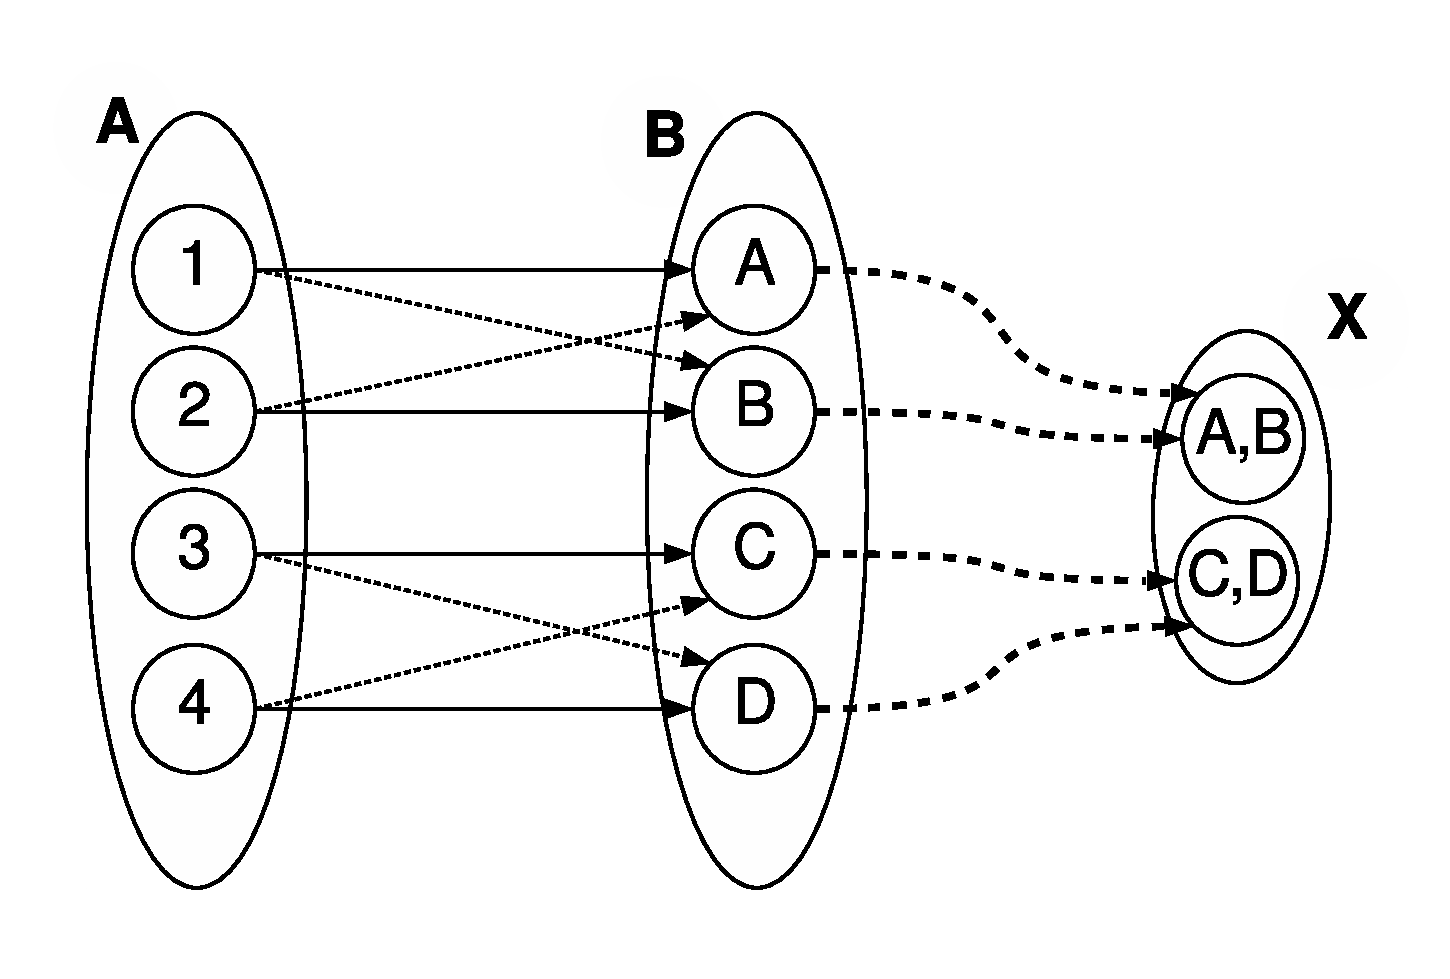
\includegraphics[scale=0.4]{images/gts/coequalizer}
  \caption{A coequalizer in \cat{Set} \important{name the morphism}}\label{fig:gts:coequalizer}
\end{figure}


\end{example}

\begin{definition}[Pushout] Given a span of arrows \mbox{$B \xleftarrow{f} A \xrightarrow{g} C$}, its \emph{pushout} is an object $X$ together with a pair of arrows \morph{f'}{C}{X} and \morph{g'}{B}{X} such that (1) \mbox{$f' \circ g = g' \circ f$} and (2) for any other object $X'$ with morphisms \morph{i}{B}{X'} and \morph{j}{C}{X'} such that $i \circ f = j \circ g$ there is a unique morphism \morph{!}{X}{X'} such that \mbox{$i =$ $! \circ g'$} and \mbox{$j =$ $! \circ f'$}.

\diagram{
  A\ar[r]^{f}\ar[d]_{g} & B\ar[d]^{g'}\ar@/^1.1pc/[rdd]^{i} &\\
  C\ar[r]_{f'}\ar@/_1.1pc/[drr]_{j}       & X\ar@{.>}[dr]^{!}&\\
                &         &X'
}

\end{definition}

\begin{example}[Pushouts in \cat{Set}] A pushout in \cat{Set} can be seen on Figure~\ref{fig:gts:pushout}. Notice that a pushout maps all elements of sets $B$ and $C$ into set $X$, ``gluing'' the ones that are identified via the morphisms \morph{f}{A}{B} and \morph{g}{A}{C}.

\begin{figure}[!ht]
  \centering
  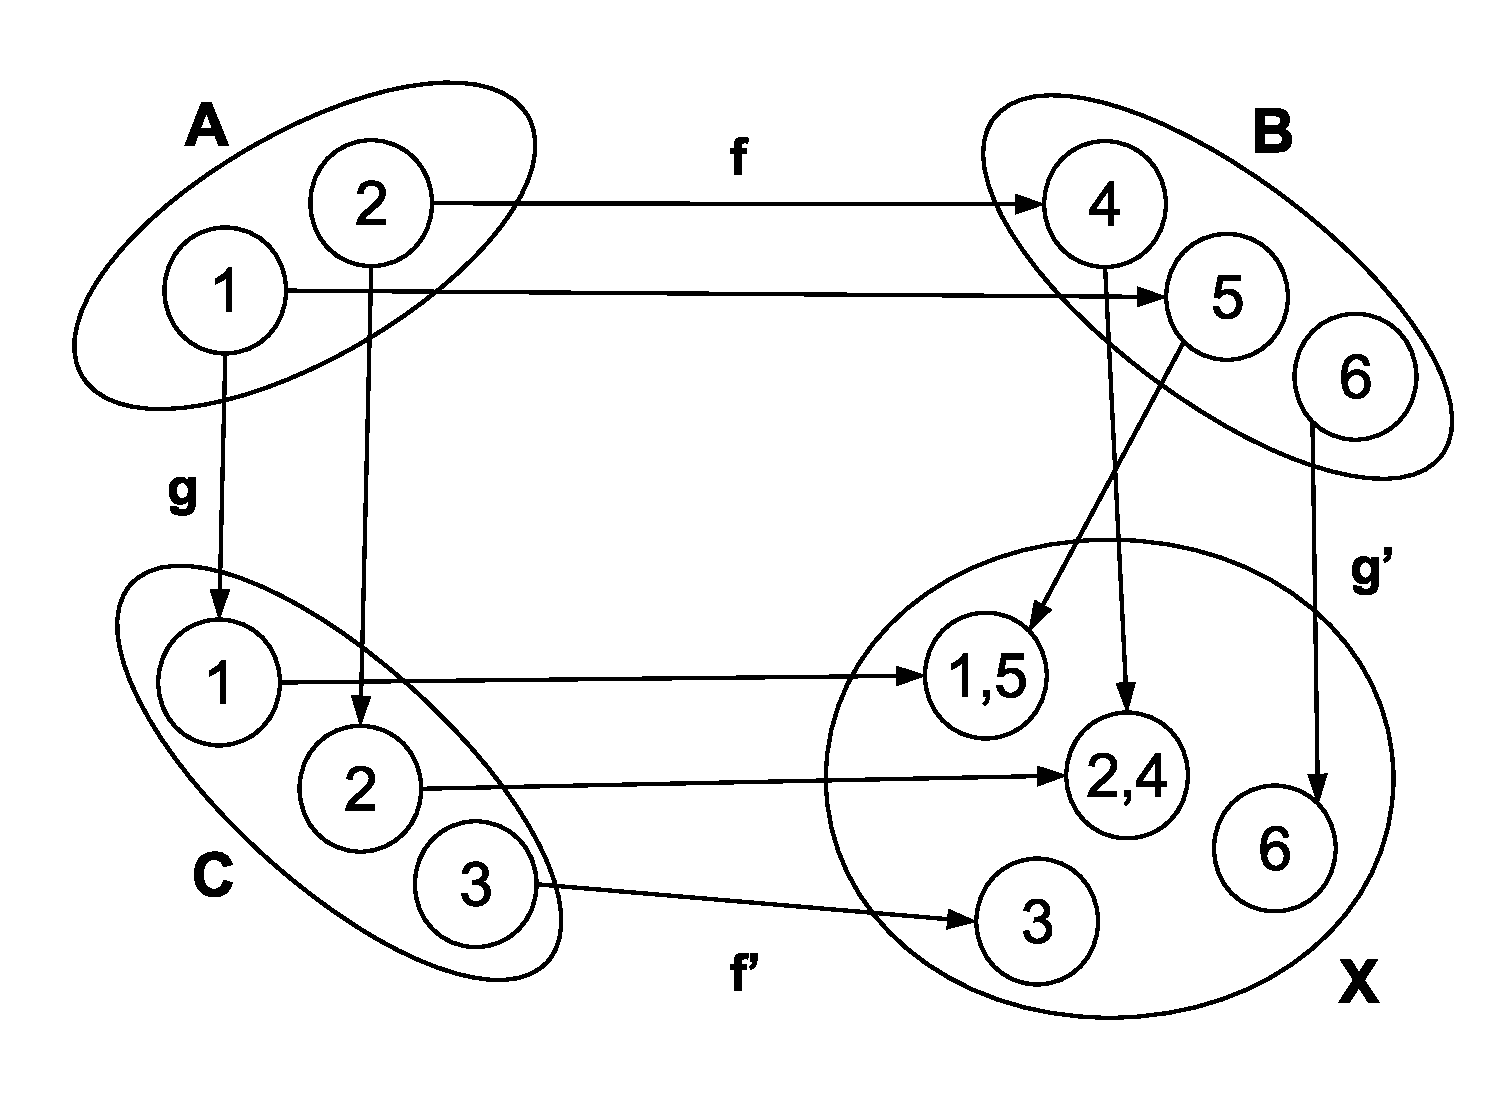
\includegraphics[scale=0.4]{images/gts/pushout}
  \caption{A pushout in \cat{Set} \important{name the morphisms}}\label{fig:gts:pushout}
\end{figure}

\end{example}

\begin{definition}[Colimit] Given a diagram $D$ in a category \cat{C}, a \emph{cocone} for $D$ is an object $X$ and a family of morphisms \morph{f_i}{D_i}{X} (one for each object $D_i$ in $D$), such that for each morphism $g$ in $D$ the outer part of the following diagram commutes.

\diagram{
  D_i\ar[rr]^{g}\ar[dr]_{f_i} &   & D_j\ar[dl]^{f_j}\\
      & X &   \\
}
\hfill

  A \emph{colimit} for a diagram $D$ is a cocone \{\morph{f_i}{D_i}{X}\} such that for any other cocone \{\morph{f'_i}{D'_i}{X'}\} there exists a unique morphism \morph{!}{X}{X'} such that the following diagram commutes for every $D_i$ in $D$.


\diagram{
  D_i\ar@/_1.1pc/[ddr]_{f'_i}\ar[rr]^{g}\ar[dr]_{f_i} &   & D_j\ar@/^1.1pc/[ddl]^{f'_j}\ar[dl]^{f_j}\\
      & X\ar@{.>}[d]^{!} &   \\
      & X'&    \\
}
\end{definition}

\begin{example}[Colimits in \cat{Set}] Colimits generalize several constructions such as disjoint unions, direct sums, coproducts, pushouts and others, where different objects of a diagram are ``glued'' together in one single object respecting commutativity. All previous examples of coproduct, coequalizer and pushout are special cases of colimits. Figure~\ref{fig:gts:colimit} shows a colimit for a diagram that can not be calculated in (one step) by any of the previous constructions.

\begin{figure}[!ht]
  \centering
  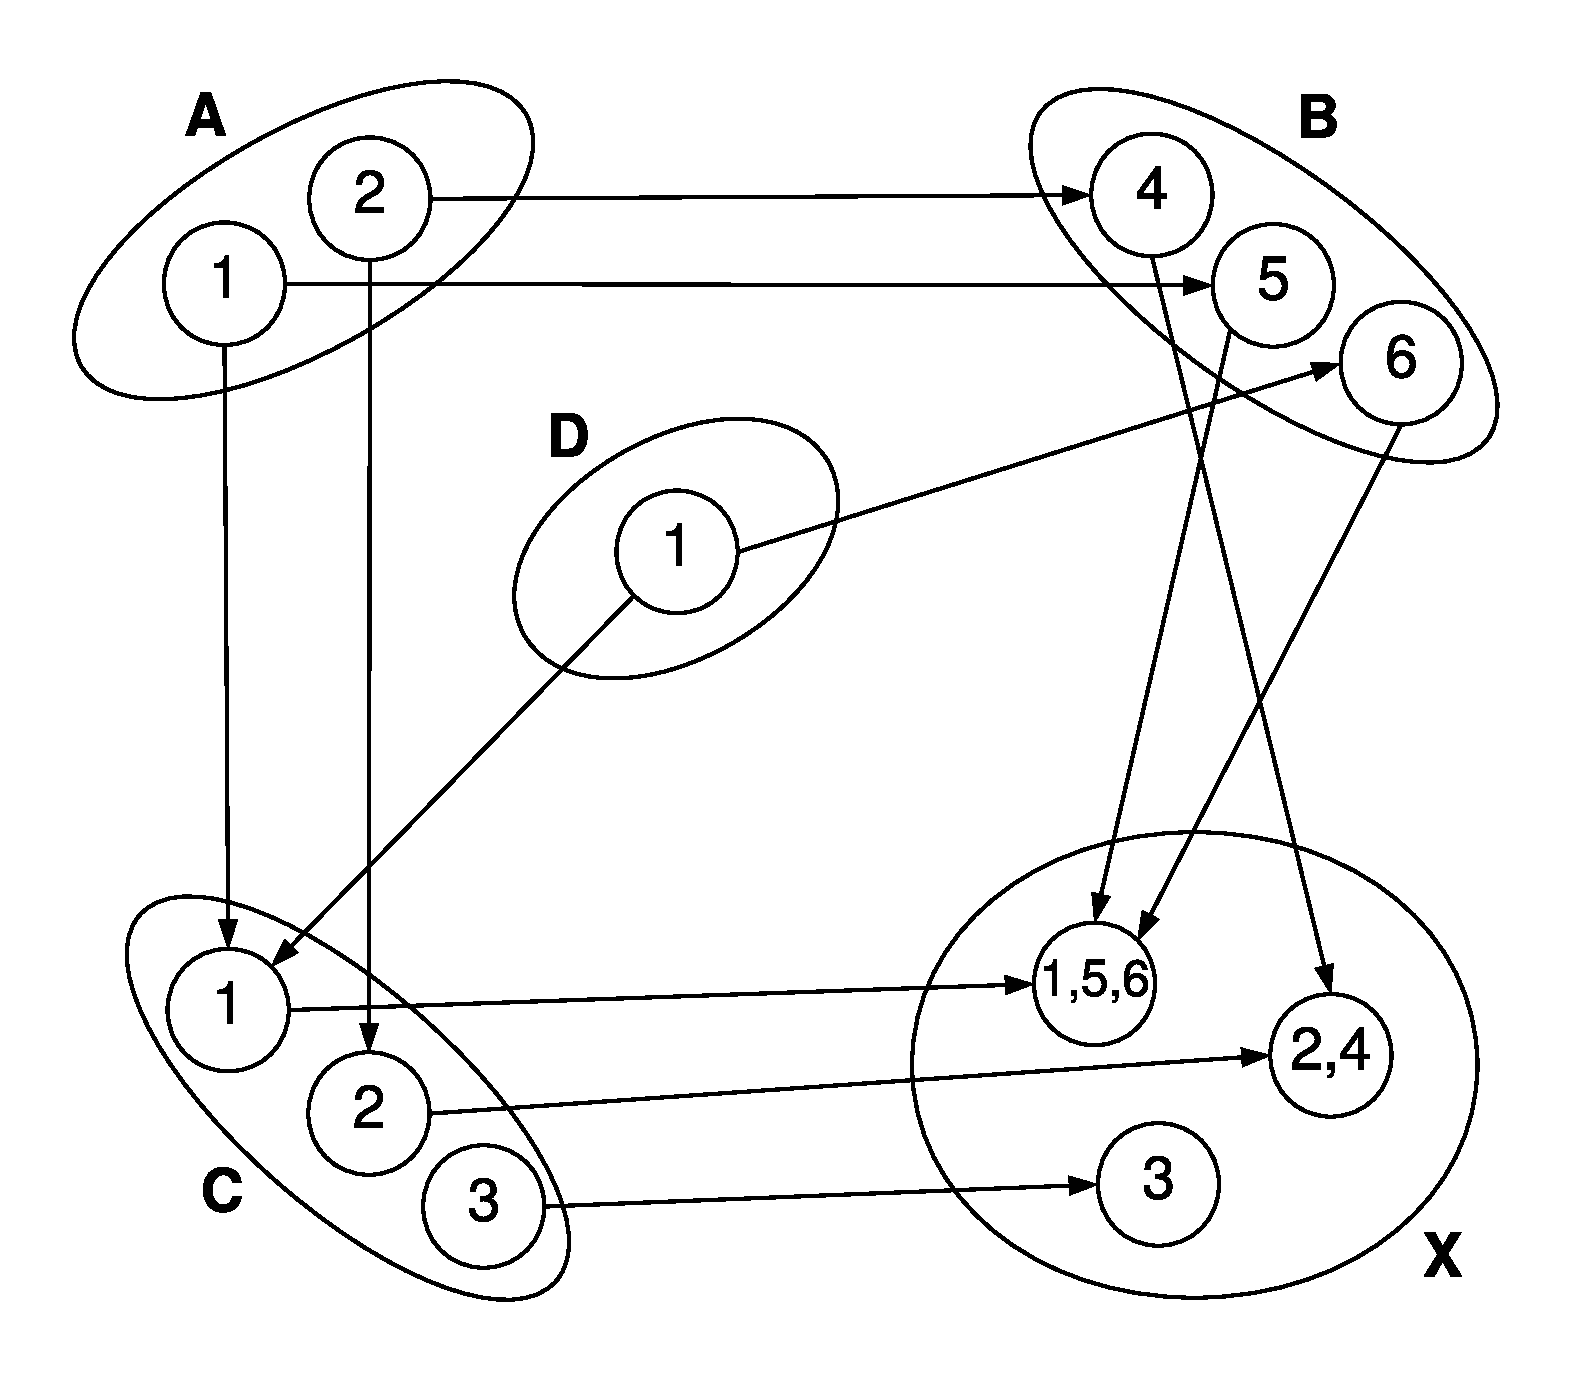
\includegraphics[scale=0.4]{images/gts/colimit}
  \caption{A colimit in \cat{Set}}\label{fig:gts:colimit}
\end{figure}

\end{example}

